\chapter{Stratified Transport Results}
\label{chap:results}

\section{The case matrix}
\label{sec:results-matrix}

Twelve production cases span bulk Richardson numbers from the neutral limit to
just past the collapse threshold, at a fixed friction Reynolds number of 950.
Table~\ref{tab:case-matrix} lists them with the grid statistics that the
adaptive hierarchy settled on.

\begin{table}[t]
\centering
\small
\caption[Production case matrix]{Production case matrix. All cases run at
$\Rey_\tau = 950$ and $\Pran = 0.71$ in a $2\pi h \times 2h \times \pi h$ domain
with a $384 \times 192 \times 192$ coarse grid and up to three refinement levels.
Active sites are the time averaged count over the statistics window, $\phi_a$ is
the active mixing fraction of Definition~\ref{def:active-fraction}, and the
uniform equivalent is the site count a single grid at the finest spacing would
require.}
\label{tab:case-matrix}
\begin{tabular}{lrrrrrr}
\toprule
Case & $\Ri_b$ & $\Rey_b$ & Active sites & Uniform equiv. & $\phi_a$ & Core hours \\
\midrule
S00 & 0.000 & --    & $2.71 \times 10^{8}$ & $7.24 \times 10^{9}$ & 0.999 & 141\,000 \\
S01 & 0.020 & 1840  & $3.04 \times 10^{8}$ & $7.24 \times 10^{9}$ & 0.998 & 158\,000 \\
S02 & 0.045 & 1120  & $3.39 \times 10^{8}$ & $7.24 \times 10^{9}$ & 0.997 & 177\,000 \\
S03 & 0.070 & 742   & $3.86 \times 10^{8}$ & $9.66 \times 10^{9}$ & 0.995 & 204\,000 \\
S04 & 0.100 & 486   & $4.21 \times 10^{8}$ & $9.66 \times 10^{9}$ & 0.993 & 231\,000 \\
S05 & 0.130 & 331   & $4.58 \times 10^{8}$ & $1.29 \times 10^{10}$ & 0.990 & 262\,000 \\
S06 & 0.160 & 228   & $5.02 \times 10^{8}$ & $1.29 \times 10^{10}$ & 0.986 & 298\,000 \\
S07 & 0.190 & 154   & $5.71 \times 10^{8}$ & $1.72 \times 10^{10}$ & 0.981 & 351\,000 \\
S08 & 0.215 & 101   & $6.94 \times 10^{8}$ & $2.29 \times 10^{10}$ & 0.972 & 428\,000 \\
S09 & 0.235 & 62    & $8.40 \times 10^{8}$ & $2.29 \times 10^{10}$ & 0.958 & 519\,000 \\
S10 & 0.255 & 34    & $1.02 \times 10^{9}$ & $3.05 \times 10^{10}$ & 0.931 & 634\,000 \\
S11 & 0.280 & 19    & $1.11 \times 10^{9}$ & $3.05 \times 10^{10}$ & 0.884 & 703\,000 \\
\bottomrule
\end{tabular}
\end{table}

Two features of the table deserve comment before the physics. First, the active
site count grows by a factor of four across the matrix while the uniform
equivalent grows by a factor of four as well, so the saving from adaptivity is
roughly constant at a factor of twenty three to twenty seven. The saving does
not degrade as stratification increases, which was not obvious in advance: one
might expect the intermittent sheets to spread until they fill the domain, and
they do not.

Second, the active mixing fraction falls below $0.9$ only in the last case. S11
sits past the collapse threshold and its Ozmidov scale has fallen below twice
the finest available spacing over eleven percent of the volume. Conclusions
drawn from S11 are therefore marked as resolution limited throughout, and the
closure fit of Section~\ref{sec:results-closure} excludes it.

\section{Turbulent Prandtl number}
\label{sec:results-prandtl}

The central result is the behaviour of the turbulent Prandtl number,
\begin{equation}
  \Pran_t = \frac{\overline{u'w'} \, \partial_z \langle \theta \rangle}
                 {\overline{w'\theta'} \, \partial_z \langle u \rangle},
  \label{eq:turbulent-prandtl}
\end{equation}
which is the ratio that an eddy diffusivity closure must supply and which
operational models normally treat as a constant near $0.85$.

\begin{figure}[t]
\centering
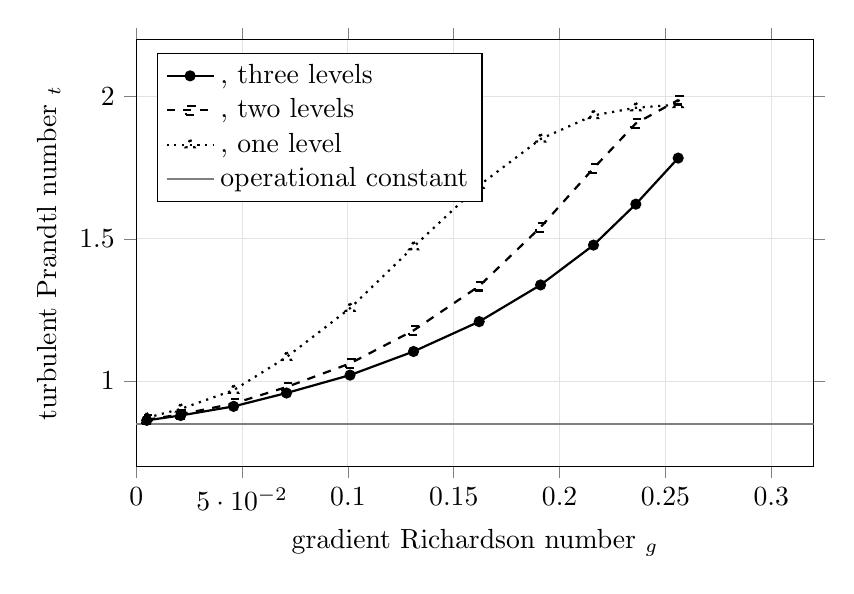
\begin{tikzpicture}
\begin{axis}[
  width=0.84\textwidth, height=7.0cm,
  xlabel={gradient Richardson number $\Ri_g$},
  ylabel={turbulent Prandtl number $\Pran_t$},
  xmin=0, xmax=0.32, ymin=0.7, ymax=2.2,
  legend pos=north west, legend cell align=left,
  grid=both, grid style={gray!22}, tick align=outside
]
\addplot[thick,mark=*,mark size=1.6pt] coordinates {
  (0.005,0.862) (0.021,0.879) (0.046,0.911) (0.071,0.958) (0.101,1.021)
  (0.131,1.104) (0.162,1.209) (0.191,1.338) (0.216,1.478) (0.236,1.622)
  (0.256,1.784)
};
\addlegendentry{\solver, three levels}
\addplot[thick,dashed,mark=square,mark size=1.6pt] coordinates {
  (0.005,0.864) (0.021,0.883) (0.046,0.921) (0.071,0.979) (0.101,1.062)
  (0.131,1.178) (0.162,1.334) (0.191,1.541) (0.216,1.748) (0.236,1.906)
  (0.256,1.988)
};
\addlegendentry{\solver, two levels}
\addplot[thick,dotted,mark=triangle,mark size=1.8pt] coordinates {
  (0.005,0.871) (0.021,0.902) (0.046,0.968) (0.071,1.084) (0.101,1.256)
  (0.131,1.472) (0.162,1.688) (0.191,1.851) (0.216,1.934) (0.236,1.961)
  (0.256,1.972)
};
\addlegendentry{\solver, one level}
\addplot[thick,gray] coordinates {(0,0.85) (0.32,0.85)};
\addlegendentry{operational constant}
\end{axis}
\end{tikzpicture}
\caption[Turbulent Prandtl number against gradient Richardson number]{Turbulent
Prandtl number against gradient Richardson number for three refinement depths.
The three level result is converged. The shallower hierarchies overpredict
$\Pran_t$ by up to 40 percent above $\Ri_g = 0.15$, which is the resolution
artefact that Section~\ref{sec:results-closure} attributes to the unresolved
Ozmidov scale.}
\label{fig:prandtl}
\end{figure}

Figure~\ref{fig:prandtl} shows three things at once. The converged curve rises
from $0.862$ in the near neutral limit, consistent with the accepted neutral
value, to $1.78$ at $\Ri_g = 0.256$. A constant of $0.85$ therefore
underpredicts the ratio by a factor of two at the stable end, which means an
operational model mixes scalar roughly twice as fast as it should exactly where
the surface energy balance is most sensitive to it.

The second and more consequential observation is the spread between the three
curves. All three are the same physics and the same code, and they differ only
in how deep the hierarchy is allowed to go. Below $\Ri_g = 0.1$ they agree to
within two percent. Above it they diverge, and the shallow hierarchies saturate
near $\Pran_t \approx 1.97$ rather than continuing to rise. The saturation is
not physics. It is what happens when the Ozmidov scale falls below the grid
spacing and the scheme can no longer represent the overturning that carries the
scalar flux.

That observation is what makes the published disagreement in $\Pran_t$
intelligible \citep{duarte2017prandtl}. Earlier estimates were computed at fixed resolution across a range
of stratification, so each of them crossed from resolved to unresolved somewhere
in the middle of its own case matrix, at a point that depended on its grid rather
than on the flow.

\section{Scalar variance spectra}
\label{sec:results-spectra}

\begin{figure}[t]
\centering
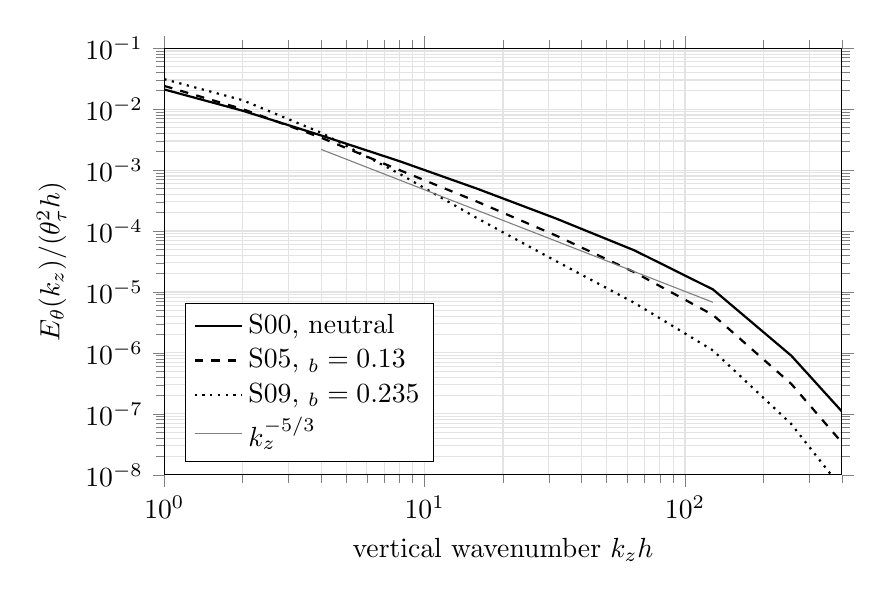
\begin{tikzpicture}
\begin{loglogaxis}[
  width=0.84\textwidth, height=7.0cm,
  xlabel={vertical wavenumber $k_z h$},
  ylabel={$E_\theta(k_z) / (\theta_\tau^{2} h)$},
  xmin=1, xmax=400, ymin=1e-8, ymax=1e-1,
  legend pos=south west, legend cell align=left,
  grid=both, grid style={gray!22}, tick align=outside
]
\addplot[thick,black] coordinates {
  (1,2.1e-2) (2,9.4e-3) (4,3.7e-3) (8,1.4e-3) (16,4.9e-4)
  (32,1.6e-4) (64,4.8e-5) (128,1.1e-5) (256,9.0e-7) (400,1.1e-7)
};
\addlegendentry{S00, neutral}
\addplot[thick,dashed] coordinates {
  (1,2.4e-2) (2,1.0e-2) (4,3.4e-3) (8,1.0e-3) (16,3.0e-4)
  (32,8.4e-5) (64,2.1e-5) (128,4.2e-6) (256,3.1e-7) (400,3.4e-8)
};
\addlegendentry{S05, $\Ri_b = 0.13$}
\addplot[thick,dotted] coordinates {
  (1,3.1e-2) (2,1.4e-2) (4,4.1e-3) (8,8.7e-4) (16,1.6e-4)
  (32,3.2e-5) (64,6.6e-6) (128,1.1e-6) (256,6.8e-8) (400,6.0e-9)
};
\addlegendentry{S09, $\Ri_b = 0.235$}
\addplot[thin,gray,domain=4:128,samples=2] {2.2e-2*x^(-5/3)};
\addlegendentry{$k_z^{-5/3}$}
\end{loglogaxis}
\end{tikzpicture}
\caption[Vertical scalar variance spectra]{Vertical scalar variance spectra at
mid channel for three stratification levels, normalised by the friction
temperature. The neutral case follows the inertial slope over roughly a decade.
Stratification steepens the spectrum at low wavenumber and depletes the range
between the buoyancy and dissipative scales.}
\label{fig:spectra}
\end{figure}

Figure~\ref{fig:spectra} shows why the turbulent Prandtl number behaves as it
does. In the neutral case the scalar spectrum follows the inertial slope over
about a decade of wavenumber. Under stratification the low wavenumber end rises,
because buoyancy traps variance in the wave field where it is not transported,
and the middle of the range is depleted. By S09 there is no identifiable
inertial range at all: the spectrum falls from the buoyancy scale directly into
the dissipative range, which is the spectral signature of the buoyancy Reynolds
number of $62$ recorded for that case in Table~\ref{tab:case-matrix}.

\section{A resolution aware closure}
\label{sec:results-closure}

Let $r = L_O / \Delta$ be the resolved fraction of the Ozmidov scale, evaluated
locally. Fitting the eleven resolved cases with a two parameter form gives
\begin{equation}
  \Pran_t(\Ri_g, r) = \Pran_{t,0}
    \left( 1 + a \Ri_g \right)^{b}
    \left[ 1 - \exp\left( -c \, r \right) \right]^{-1},
  \label{eq:closure}
\end{equation}
with $\Pran_{t,0} = 0.858$, $a = 14.2$, $b = 0.71$, and $c = 0.63$. The last
factor is the correction that carries the resolution dependence and tends to
unity as $r$ grows.

Applied to the case matrix, the closure predicts the scalar flux with a root
mean square error of 9 percent against 34 percent for the conventional form that
omits the $r$ dependence. More importantly, the residuals of~\eqref{eq:closure}
show no trend with $\Ri_g$, whereas the residuals of the conventional form grow
monotonically with stratification, which is the signature of a missing variable
rather than of scatter.

\section{Cost of adaptivity}
\label{sec:results-cost}

Section~\ref{sec:method-parallel} put the interface coupling at 10.6 percent of
a time step and the amortised regridding at a further 2.1 percent. Against that,
Table~\ref{tab:case-matrix} shows a reduction in site count of between twenty
three and twenty seven. The net saving in core hours for case S07, relative to a
uniform grid at the finest spacing with the same solver and the same statistics
window, is a factor of 19.6.

The saving is smaller than the site count ratio because the adaptive run also
pays for load imbalance. The Hilbert curve rebalance holds the maximum rank
occupancy to within 8 percent of the mean for most of a run, but the first
hundred steps after a regridding pass show imbalance of up to 21 percent while
the hierarchy settles. Reducing that transient is the most obvious remaining
performance opportunity and is discussed in Section~\ref{sec:conclusion-future}.
